\documentclass{article}
\usepackage{default} 
\usepackage{graphicx}
\usepackage{tipa}
\usepackage{lingsty}
\usepackage{gb4n}
\usepackage[noload]{qtree}
\usepackage{ipashortcuts}
\usepackage[authoryear]{natbib}
\bibpunct[:]{(}{)}{,}{a}{}{,}
\setlength{\bibsep}{0.05cm}
\usepackage{multirow}
\usepackage{array}
\usepackage{subcaption}
\usepackage{url}
\newcommand{\R}{\textipa{\textsubbar{r}}}
\newcommand{\tamzh}{\textipa{\textsubbar{l}}}
\usepackage[tableposition=top]{caption}

\usepackage{float}
\floatstyle{plaintop}
\restylefloat{table}

\renewcommand{\lz}{LZipa}
\renewcommand{\tz}{TZipa}
\renewcommand{\dz}{DZipa}
\renewcommand{\nz}{NZipa}
\renewcommand{\ng}{NGipa}
\renewcommand{\und}{UNDipa}
\renewcommand{\dentt}{DENTT}
\renewcommand{\dentd}{DENTD}
\renewcommand{\phonem}{PHONEM}
\renewcommand{\xref}[1]{(\ref{#1})}
\renewcommand{\ea}{()\\}
\renewcommand{\phonet}[1]{[\textipa{#1}]}
\renewcommand{\phonem}[1]{/\textipa{#1}/}
\renewcommand{\graphem}[1]{\textlangle#1\textrangle}
\renewcommand{\zero}{\ensuremath{\emptyset}}
\renewcommand{\lt}{$<$}
\renewcommand{\gt}{$>$} 
\renewcommand{\trs}[2]{{\em #1\em} `#2'}
%opening
\title{Catch me if you can: Pathways of Dravidian influence in Sri Lanka Malay}
\author{Sebastian Nordhoff}


\begin{document}

\maketitle
 
\begin{abstract}
 Discussions of the history of Sri Lanka Malay have so far tried to evaluate  the development of   Sri Lanka Malay with regard to the relative influence from the adstrates Sinhala and Tamil. This paper shows that such an approach is too coarse-grained and that the dialectal situation of especially Tamil has to be taken into account. After an overview of the dialectal situation we find on the island, three directions of language change are established: 1) Sinhala moves towards a general Tamil typology; 2) South Western Muslim Tamil moves towards Sinhala; and 3) Sri Lanka Malay moves towards South Western Muslim Tamil and/or Sinhala. A discussion of the  problematic nature of the assumptions of `fixed targets' in language contact studies emanating from point 3) closes the paper. 
\end{abstract}

\textbf{Keywords: Sri Lanka, Sri Lanka Malay, Sinhala, Tamil, dialectology, language contact}

\section{Introduction}
Sri Lanka Malay is the language of the descendants of immigrants (mostly soldiers) brought to Sri Lanka by the colonial powers of the Dutch (1656-1796) and British (1796-1948). It is the most divergent variety of Malay and has adopted a thorough South Asian typology with retroflexes, bound morphology, head-final word order and vector verbs. 

It is clear that these structures were acquired in the roughly three centuries  between the Dutch period and now. A more contentious question is whether the development of these structures is due to (Moorish) Tamil or Sinhala influence. Proponents of Sinhala hold that 80\% of the population speak Sinhala, while Moors only make up 6\% of the population. Defendants of Tamil influence reply that the Moors had close cultural, religious and familial ties with the Malays, which gave their language a higher impact than numbers alone would suggest. 

The debate has so far pitched ``Sinhala'' against ``Tamil'', treating them as inert monoliths. As a first approach, this is eminently sensible, but a closer look reveals that there are a number of language change processes going on \em within \em these blocks, which one has to consider when analyzing the structure of Sri Lanka Malay.

Sri Lanka Malay has adopted many structures which are typically Dravidian. The question which arises is \em how \em these structures made their way into the language. In order to address this issue, I will proceed as follows: 
I will start with an overview of the linguistic ecology of Sri Lanka in Section \ref{sec:ecology}.
Section \ref{sec:dravidianfeatures} will illustrate some of the typological characteristics Sri Lanka Malay acquired through language contact.
I will present new findings on language contact in Section \ref{sec:languagecontact} 
and discuss them in Section \ref{sec:discussion}.


% \section{Convergence}
% Convergence is generally seen as two languages becoming more like another. \citet{Mattheier1996}, however, holds that in many cases, it is better to speak of `advergence', as there is usually one language which changes a lot in the direction of the other, while the other changes hardly at all. 
% 
% A clear case of advergence would be Pennsylvania Dutch, which becomes more like English, whereas the surrounding varieties of English are hardly influenced by Pennsylvania Dutch. A clear case of convergence would be Kupwar \citep{GumperzEtAl1971}, where all three languages (Urdu, Kannada, Marathi) underwent change in the direction of the others. 
% 
% In this paper, I want to discuss language change processes in Sri Lanka and show that, depending on the subvarieties,  there are multiple advergence processes going on in conflicting directions. This network of changes makes it difficult to exactly locate the origin of a change. For instance, Sinhala, at a broad level, converges towards Tamil. Certain (Muslim) Tamil dialects, however, converge towards Sinhala. Sri Lanka Malay, finally, converges towards these Muslim Tamil dialects. If we find  a feature X in Sri Lanka Malay, how can we say whether it comes directly from Tamil, whether it comes from Tamil via Sinhala, or whether it comes from Sinhala via Muslim Tamil? 
% 
% This paper is structured as follows: I will first give an overview of the Sri Lankan linguistic ecology, sketching the sociolinguistic, geographic and demographic setup of the relevant languages and giving some historical background. I will then discuss received wisdom about the contact situation. After taking a look at the dialectology of the respective languages, I will reassess the contact situation, showing that the language change processes are more complex than assumed. 

\section{The Sri Lankan linguistic ecology} \label{sec:ecology}
The first language spoken in Sri Lanka that we know of is the \textbf{Vedda} language \citep[505]{Geiger1973}. Various proposals have been made as to its origins, but as a matter of fact, language attrition has proceeded to a point where little of any substance can be said about the affiliation of this language. 
% Genetic studies suggest that the Vedda people are related to populations of Andaman and Nicobar. Vedda as spoken today can be considered a variety of Sinhala with some lexical and morphological peculiarities \citep{abc}. Due to the lack of material, Vedda will not be considered further in this paper. 


\begin{figure}
\begin{center}
\begin{subfigure}[b]{.4\textwidth}{ 
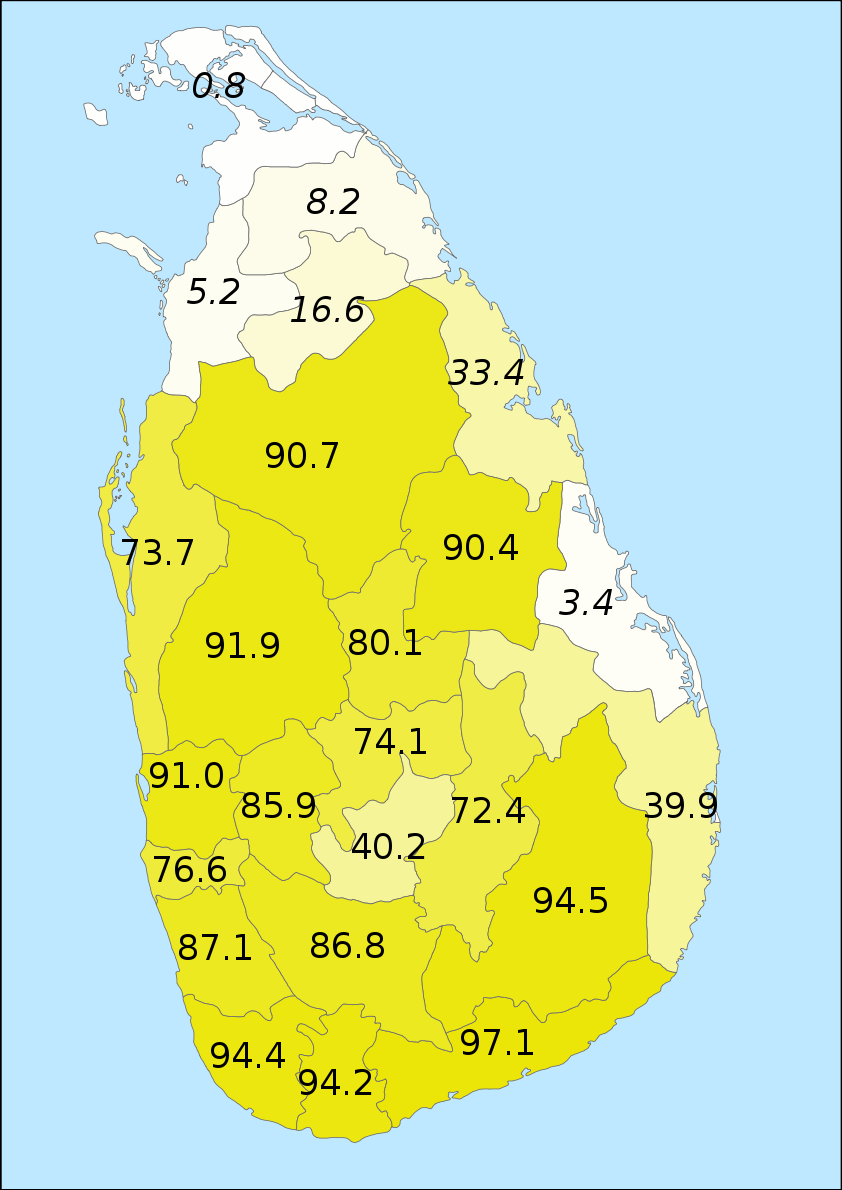
\includegraphics[width=\textwidth]{SriLankaSinhalese.png}
\caption{Sinhala}
}
\end{subfigure}
\begin{subfigure}[b]{.4\textwidth}{ 
 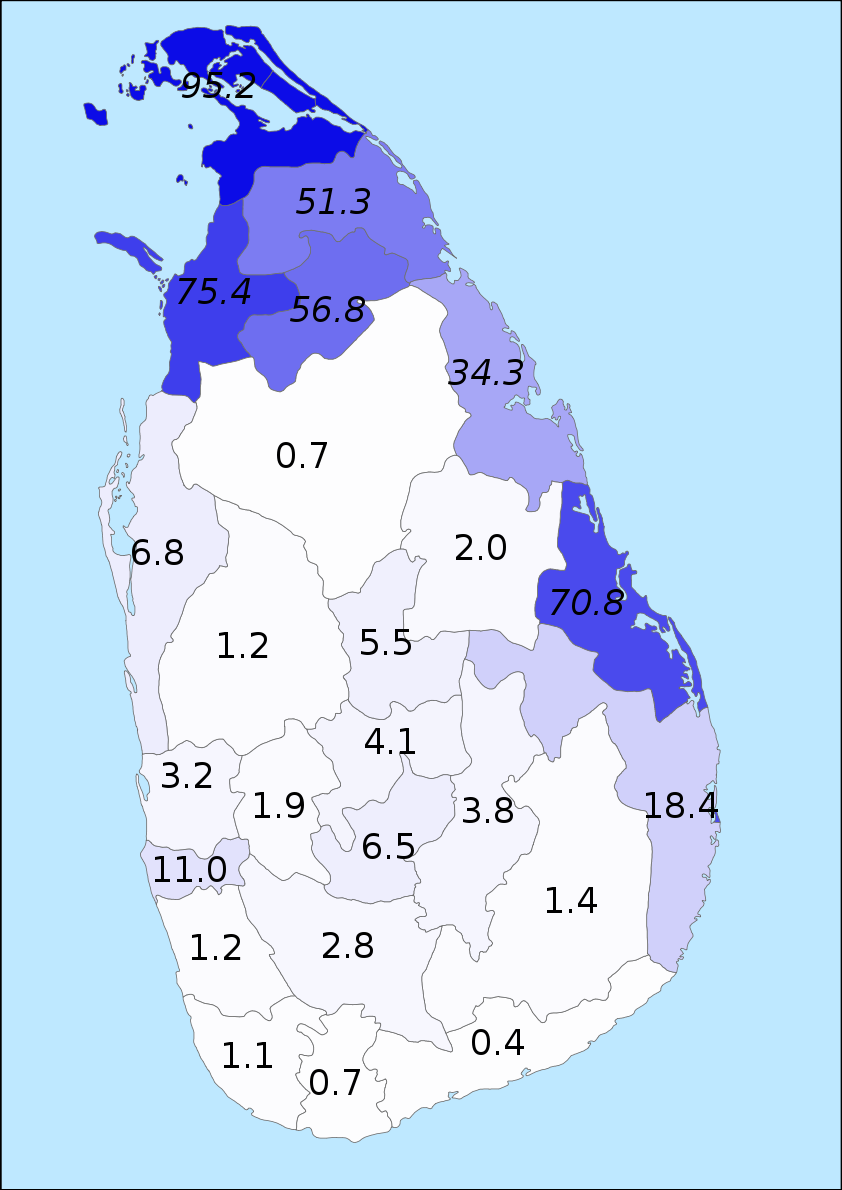
\includegraphics[width=\textwidth]{SriLankaNativeTamil.png}
\caption{Ceylon Tamil}
}
\end{subfigure}
\begin{subfigure}[b]{.4\textwidth}{ 
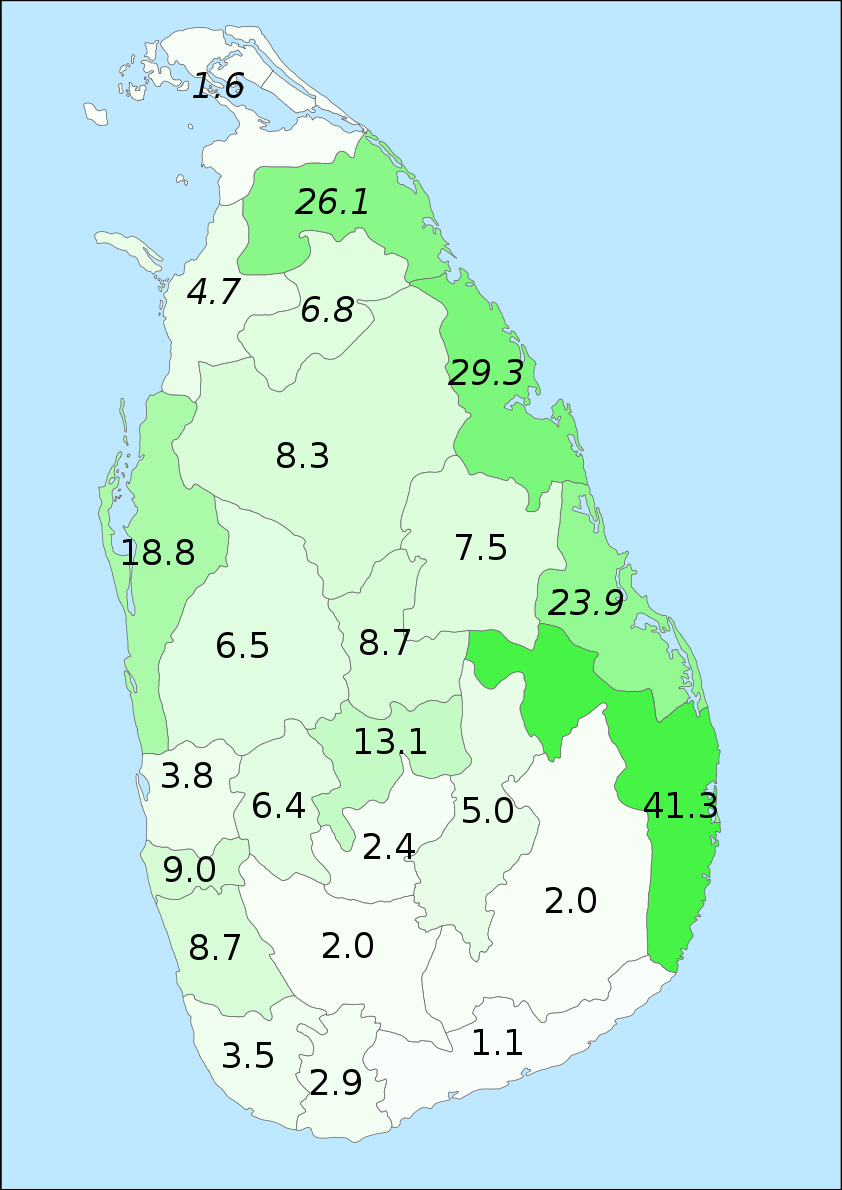
\includegraphics[width=\textwidth]{SriLankaMoor.png}
\caption{Moorish Tamil}
}
\end{subfigure}
\begin{subfigure}[b]{.4\textwidth}{ 
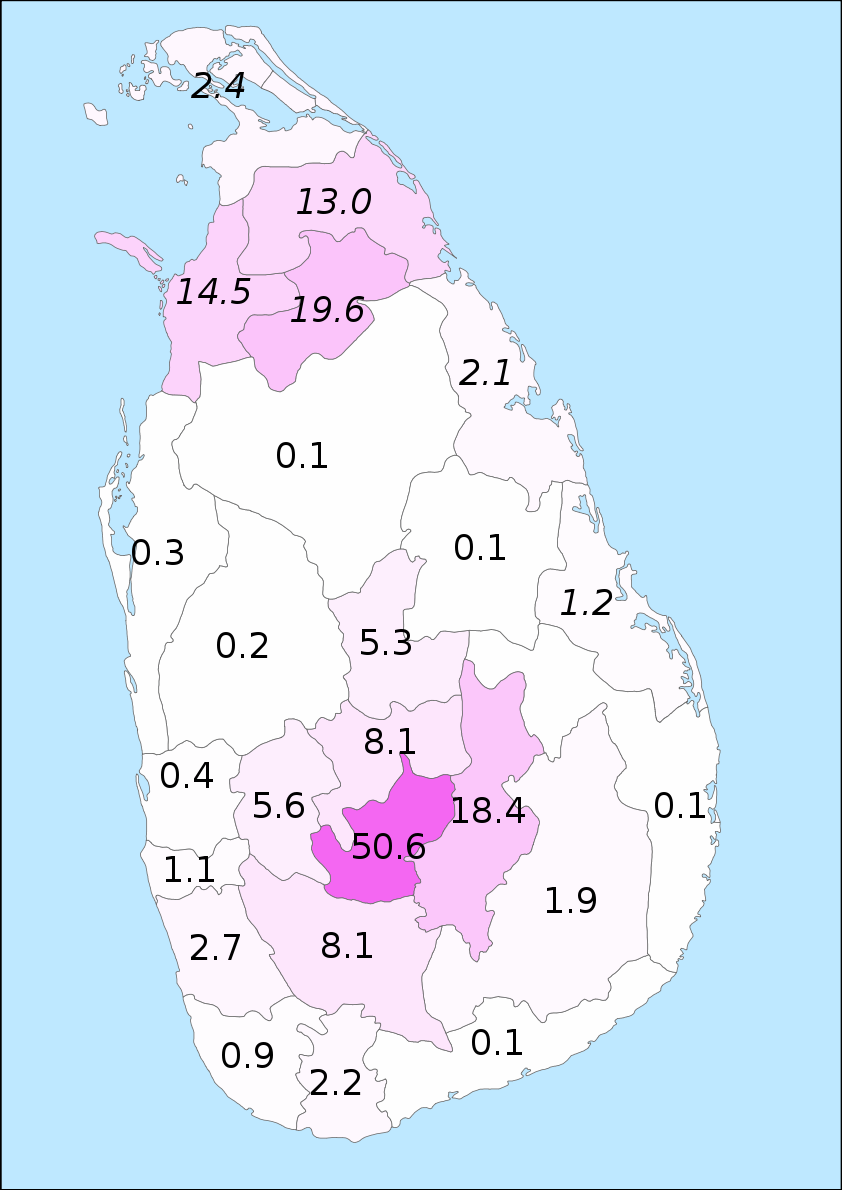
\includegraphics[width=\textwidth]{SriLankaIndianTamil.png}
\caption{Indian Tamil}
}
\end{subfigure}

\end{center}

 \caption{The current distribution of linguistic groups in Sri Lanka. Based on census data from 2001 and 1981.  \\{\tiny
{http://commons.wikimedia.org/wiki/File:Sri\_Lanka\_Moor.svg};    
{http://commons.wikimedia.org/wiki/File:Sri\_Lanka\_Sinhalese.svg};  \\
{http://commons.wikimedia.org/wiki/File:Sri\_Lanka\_Indian\_Tamil.svg};  
{http://commons.wikimedia.org/wiki/File:Sri\_Lanka\_Native\_Tamil.svg}.   \\
All files CC-BY 2.5 Sadalmelik.}
 }
\end{figure}

Sinhala (Indo-Aryan) and Tamil (Dravidian) both arrived on the island about three millennia ago, although the respective order of arrival is a matter of debate \citep[4]{Gair1998}. Sinhala has been shown to share some features with Western Indo-Aryan languages like Marathi and others with Eastern Indo-Aryan languages like Bengali \citep{Geiger1973}. This suggests two waves of immigration, but again the chronological order is unsure (Figure \ref{fig:migrationISL}). 



\begin{figure}
\begin{center}
 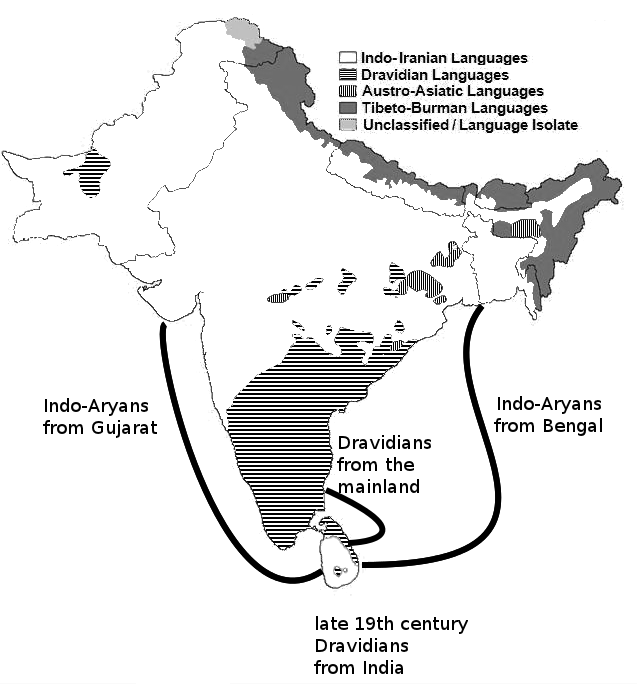
\includegraphics[height=.4\textheight]{insl2.png}
\end{center}
 \caption{Migrations from India to Sri Lanka. \\{\tiny based on http://commons.wikimedia.org/wiki/File:South_Asian_Language_Families.jpg CC-BY-SA-3.0-MIGRATED http://commons.wikimedia.org/wiki/User:BishkekRocks}}
\label{fig:migrationISL}
\end{figure}


\textbf{Sinhala} is separated from its Northern cousins by the Dravidian languages of South India and is isolated within the family.\footnote{Disregarding
 Dhivehi (Maldivian), which is an offshoot of Sinhala.
}
Due to prolonged contact with Dravidian languages, Sinhala became much more Dravidianized than any other Indo-Aryan language. 
% In fact, the Indo-Aryan nature of Sinhala is so well concealed that in the 19th century, \citep{Rask1821} classified Sinhala as a Dravidian language. 
In the 19th century, there was some debate as to whether Sinhala was actually Dravidian or Indo-Aryan, but Geiger established the Indo-Aryan nature of Sinhala beyond doubt. 

\citet{Gair1994ssala,Gair2012xc} adds Sinhala to the South-South Asian Sprachbund, which comprises Southern India, Sri Lanka, and the Maldives. Features which set off Sinhala from the Northern Indo-Aryan languages are absence of aspirates, long \=e and \=o, conjunctive participles without a same-subject requirement, evidentials, quotatives, and a very thorough left-branching structure. These features are shared with Tamil.

Sinhala is today the majority language of Sri Lanka with about 74\% of the population speaking it as first language. Sinhala speakers are Buddhists or Christians. They mainly live in the West, Center, and South of the island, but can be found elsewhere as well. After the end of the Sri Lankan Civil War, there are ideas of settling Sinhala speakers in the Northern regions as well, which are predominantly Tamil.


\textbf{Sri Lankan Tamil} prides itself as a very old and pure form of this language. Tamil is spoken by the Sri Lankan Tamils (Hindu or Christian) mainly in the North, the Moors (Muslim) in the West and in cities, and the Indian Tamils (Hindu or Christian) in the central tea estates and the North. These varieties differ considerably. Altogether, about 25\% of the Sri Lankan population speak one variety or another of Tamil as their mother tongue. 
Sri Lankan Tamil uses the same script and orthography as Indian Tamil, but spoken Sri Lankan Tamil is not intelligible to speakers from India. The differences are so important that speakers from India frequently think that their interlocutor does not speak a variety of Tamil at all, but rather Malayalam. It should also be noted that Tamil is a diglossic language, and that written Tamil differs considerably from any variety of spoken Tamil. 

Jaffna Tamil is the most prestigious variety of Tamil on the island. Its main features are archaic phonology and morphology, a threefold deictic contrast, and a more differentiated negation system than Indian Tamil. The other varieties of Tamil on the island tend to be eclipsed by Jaffna Tamil in scholarly domains. We will return to this below. 

\textbf{Sri Lanka Portuguese} arrived on the island during the Portuguese period (1503-1656) as a Creole. Due to intermarriage with the local population, the language became thoroughly Lankanized and is now the only Creole with a European lexifier to have thorough SOV word order or postpositions. The Dutch (1656-1798) continued to use Sri Lanka Portuguese as a lingua franca, a practice which continued into the early days of British rule (1798-1948). As a lingua franca, Sri Lanka Portuguese was also acquired by populations which otherwise had no connections to the colonial administration. Today, Sri Lanka Portuguese is spoken on the East Coast (Tamil-dominated) by about 4000 Portuguese Burghers, and by a very small number of Sri Lankan Kaffirs (descendants of slaves) on the West Coast. \citet{Smith1979} shows that the Burghers' Sri Lanka Portuguese is thoroughly influenced by Tamil. A recent overview can be found in \citet{Nordhoff2013slp}.  %\citet{Hettiaratchi} refers to a recording of a centenary speaker 
of Sri Lanka Portuguese in the Sinhala dominated region, 
% whose speech shows more influence from Sinhala. 


\textbf{Sri Lanka Malay} is the language of the descendants of immigrants brought during the Dutch and British period. It was mainly spoken in the centers of colonial administration, i.e. cities and towns in the center and in the South. Towards the end of the 19th century \citep{Hussainmiya1990}, Sri Lanka Malays were also employed as overseers on the emerging tea estates in the central Hill Country. Sri Lanka Malay has been argued to show influence from Muslim Tamil \citep{SmithEtAl2006cll} and/or from \textsc{Sinhala} \citep{Ansaldo2008genesis}. 

Sri Lanka Malay is relatively homogeneous. There is a small pocket of Sri Lanka Malay speakers on the South coast (Kirinda and Hambantota) which has some dialectal peculiarities, but overall mutual intelligibility is good. 

% \textbf{Sri Lankan English} is the last language to develop on the island. It has mostly been treated within sociolinguistics. Studies of Sri Lankan English have focused on the Colombo variety, influenced by Sinhala. Work by \citet{Kumaraswamy} shows, that Sri Lankan English as spoken by Tamils differs from the variety portrayed in most linguistic work.
% Besides a peculiar phonology and lexical influences from the local languages, the syntax of Sri Lankan English has also been heavily influenced by the local languages.

% \section{Language contact and change in Sri Lanka}
The standard view about language contact in Sri Lanka is that all languages that get there converge towards Tamil. This assumption is based on the observation that Sri Lankan Tamil is an archaic variety \citep{Zvelebil1959II}, which suggests that it has not changed a lot. Given that Sri Lanka is a sprachbund \citep{Bakker2006}, potentially within a larger South-South-Asian Sprachbund \citep{Gair2012xc}, the logical conclusion is that all other members have converged to the most conservative language, Tamil in this case. This is received wisdom for \textsc{Sinhala} \citep{Geiger1973, Elizarenkova1972}, Sri Lanka Portuguese \citep{Smith1979} and Sri Lanka Malay \citep{Hussainmiya1990, SmithEtAl2006cll, Bakker2006}.  



\section{A closer look at the contact situations}
While at first sight, it appears that Tamil provides the typological sink all languages of the island move towards to, a closer look at the actual varieties in question casts doubt on this scenario. I will now delve deeper into the internal diversity of the languages of the island and show that  the language change processes are far more complex than presented beforehand. 



\subsection{Sinhala}

Sinhala is quite homogeneous as a language. ``We can hardly speak of any dialectal difference of the Sinhalese language in the Island itself'' \citep[168]{Geiger1938}.\footnote{\citep[also cf.][xii]{Jayawardena1996}.} This is especially true if we compare it with the wealth of Tamil dialects on the island (see below).\footnote{These remarks are concerned with diatopic variation of the spoken language. As an anonymous reviewer points out, due to diglossia, there is obviously diastratic variation with the written language.}

Tamil influence on Sinhala syntax is clear and widely accepted. It is most obvious in  dependent structures. \citet{Gair1998someremarks} states   ``[S]ubordinate verbal structures as a whole are of a strikingly Tamil and Dravidian character ...  the cumulative effect is nothing short of overwhelming.'' 

The phonological features of long mid vowels and lack of aspiration also distinguish Sinhala from Northern Indo-Aryan languages, and make it appear closer to Tamil. This led \citet{Elizarenkova1972} to argue for an extensive phonological influence from Tamil on Sinhala.\footnote{Elizarenkova gives more features which argue for Tamil influence, but they are all empirically problematic. }

In a very detailed study, however, \citet{Gair1985dravidianization}, drawing on material by \citet{Karunatillake1969}, shows that all the mentioned changes towards Tamil are either empirically problematic or were accompanied by changes \em away \em from Tamil in the very same periods.  For instance, long /e/ and /o/ in Sinhala developed after the eighth century BC. This looks like Tamil influence, since Tamil has this distinction as well. However, \em before \em the eighth century, Sinhala had lost all vowel length distinctions altogether. This is a most un-Tamil development. A movement away from Tamil would then be immediately followed by a movement towards Tamil. It is of course possible that the sociodemographic setting changes a lot in short time, and that patterns of language change follow. However, Gair shows that the phonological history of Sinhala is such that movements towards Tamil are usually immediately followed by movements away from Tamil. This would entail a flickering sociodemographic setting,
 
where Tamil 
influence 
is turned on and off in very short intervals, an unlikely explanation. 


As for the lexicon, Tamil influence is beyond doubt. The same is true for syntax. \citet{Gair2012xc} lists the following features which point to clear Tamil influence in Sinhala:\footnote{It is not clear how this influence in morphosyntax could be reconciled with the claimed absence of influence in phonology.}

\begin{itemize}
 \item Question marker appears at the end of sentence (postverbal) as the unmarked location, but may also occur on questioned sentence-internal constituents
 \item  Subordinate clauses marked at the end, by a verbal affix or a conjunctive form of some kind, rather than by initial conjunctions (which are rare or missing altogether except for sentence adverbs) 
 \item Preposed relative clauses (adjectival sentences) as the only or main alternative. 
 \item Correlatives use a WH-word rather than a correlative form of the Indo-Aryan type and are generally restricted to indefinite or conditional contexts and commonly employ a sentence particle (dubitative or question) on the subordinate clause. 
 \item  Sentence-final quotative from `say' 
 \item  Sentences may be nominalized without genitivization (or deletion) of subject, by employing a sentence-final form or verbal affix. 
 \item  Focused (nominal cleft) sentences, including those with rightward focus. 
 \item   Negatives: 
  \begin{itemize} 
    \item    Negative varies with type of main clause (verbal, equational, existential). 
    \item   Negative verbs in subordinate clauses. 
    \item   Cleft sentences negated like nominal equational ones. 
  \end{itemize}

 \item  Conjunctive participles may occur with overt lexical subjects, not co-indexed with main subject (or agent). [Extent yet to be determined] 
 \item A sentence-final reportative or hearsay particle (unrelated to the quotative). 
\end{itemize}
 


\subsection{Tamil}
The internal diversity of Tamil is very high. The first division to be made is between written Tamil and spoken Tamil: Tamil is a diglossic language. There are a number of good grammars of the written language, the spoken language has received less attention. In the context of this paper, written Tamil is not relevant. Spoken Tamil  can be divided into Indian Tamil (with further subdivisions) and Sri Lankan Tamil (See Figure \ref{fig:tamildialects}). There are some descriptions of Standard Spoken Indian Tamil \citep{Lehmann1989tamil,
Schiffman1999}, but the overall description of dialects is dire \citep{Pillai1986}. Furthermore, the Indian Standard does not transpose to Sri Lanka. \citet{Schiffman1999} notes: 
\begin{quote}
 In Sri Lanka, the notion of accepting or not accepting  the ``unifying'' ability of S[tandard] S[poken] T[amil] is another matter, since SST is understood but not accepted as an intercaste mode of communication among Sri Lankan Tamils. This matter will not be resolved until the civil war in that island has ended.
\end{quote}
Note that Sri Lankans can understand the Indian standard, but the reverse is not true.  


 

\begin{figure}
\begin{center}
\Tree [.Tamil 
	{Written\\Tamil} 
	[.{Spoken\\Tamil} 
			  [.{Indian\\Tamil} 
			    {Continental\\Indian Tamil} {Sri Lankan\\Estate\\Indian Tamil} ]
			  [.{Sri Lankan\\Tamil}  
			    [.{Hindu/Christian\\Tamil} Negombo Jaffna Trincomalee Batticaloa ]
			  [.{Muslim\\Tamil} {NE\\Muslim\\ Tamil} {SW\\Muslim\\Tamil} ] 
] !\qsetw{8cm}  
] !\qsetw{3.5cm} 
] 
\caption{Dialectology of Tamil with special focus on Sri Lanka}
\label{fig:tamildialects}
\end{center}
\end{figure}
 
Within Sri Lanka, further subdivisions can be made.   \citet[170f]{Gairdonotuse} state: ``There is, in fact, more dialect variation within  Tamil in Sri Lanka than there is within the majority (Indo-Aryan) language Sinhala.''
 

Within Sri Lanka, the most prestigious variety is Jaffna Tamil \citep{Zvelebil1959II,Kuiper1962,Pillai1962,Zvelebil1966,Gairdonotuse,GairEtAl2005spokenTamil, Suseendirarajah1993}, spoken by Hindus and Christians. \citet[137]{Zvelebil1966} notes:  ``It happens  quite frequently that, when speaking about  Ceylon(ese) Tamil, what authors have really in mind is (one dialect of) \em Jaffna \em Tamil. This should of course be avoided.'' Next to Jaffna Tamil, the varieties of Trincomalee \citep{Zvelebil1959I,Zvelebil1966} and Batticaloa \citep{Zvelebil1966,Batticaloa} also deserve mention. These varieties can clearly be distinguished. Tamil as spoken by Muslims differs from the variety used by the Hindus and Christians. Muslim Tamil itself is divided into a North-Eastern variety, close to Batticaloa Tamil, and a South-Western variety, which is heavily Sinhalized \citep{Nuhman2007}. \citet{Zvelebil1959II,Zvelebil1966} also mentions `Mixed Common Ceylonese' as a (then) developing standard \citep[
also cf.][]{
GairEtAl2005spokenTamil}.


Another Sinhalized variety is Negombo fishermen's Tamil \citep{Bonta2004,Bonta2010}, which, like South-Western Muslim Tamil has lost verbal agreement. 

Things are further complicated by Indian migrant workers in the central tea estates and the Northern provinces, who arrived in the late 19th century. They spoke Indian dialects of Tamil (and other Dravidian languages), and their speech today is still closer to Indian Tamil than to Sri Lankan Tamil. \citet{Gairdonotuse} mention onglides and syncopation as mainland features found in Estate Tamil.  Among these dialects, processes of dialect leveling probably took place \citep{Wijeratne2005}, but this is in need of further research. 

As far as language change is concerned, the varieties of Jaffna, Trincomalee and Batticaloa are generally seen as archaic, with little or no change towards Sinhala having taken place. All varieties of Muslim Tamil show Arabic influence in the lexicon \citep{Nuhman2007}, and South-Western Muslim Tamil and Negombo fishermen's Tamil (non-Muslim) show syntactic and phonological influence from Sinhala. \citet{Bonta2010} reports that the following features point towards Sinhala influence in Negombo Fishermen's Tamil. 

\begin{itemize}
 \item loss of verb agreement{$\dag$}
 \item first person present tense denotes strong intention
 \item changes in the semantics of the morphological future 
 \item existential used for possibilitative 
 \item reduplication denotes progressive{$\dag$}
 \item changes in negatives
 \item (re)development of a three way deictic system{$\dag$}
 \item calque of an emphatic construction 
 \item `at night' formed with the dative {$\dag$}
 \item infinitive + existential for debitive{$\dag$}           
\end{itemize}

The features marked with a dagger {$\dag$} are also found in Sri Lanka Malay. Depending on the variety we look at, Tamil influence in Sri Lanka Malay therefore would vary greatly. The Negombo fishermen dialect is described quite extensively in the relevant domains, and shows to what extent non-standard varieties of Tamil can be Sinhalized. It is clear from the socio-demographic setting (professional occupation, region, religion) that Negombo fishermen's Tamil did not exert influence on Sri Lanka Malay. Still, it can provide some insights on the extent of possible Sinhalization of other dialects of Tamil. A case in point is South-Western Muslim Tamil. There is consensus that this variety is a highly relevant contact language for Sri Lanka Malay, but it is described in less detail than Negombo fishermen's Tamil. A number of interesting parallels, however, emerge from the literature. \citet[72-79]{Nuhman2007} notes:

\begin{itemize} 
 \item lexical differences in religious vocabulary
 \item frequent initial voiced plosives (S,{$\dag$})
 \item geminate voiced plosives (S,{$\dag$})
 \item absence of retroflex liquids (S,{$\dag$})
 \item clearer articulation of vowels (S,{$\dag$})
 \item lack of agreement (S,{$\dag$}). See Table \ref{tab:TAMagr}
 \item different causative marker; different simultaneity marker
 \item of 55 kin terms, 25 are shared and 30 are different between the NE and the SW variety 
 \item Sinhala lexical borrowings (S)
\end{itemize}

An (S) in this enumeration points to features where an explanation involving Sinhala is possible. The dagger denotes, as above, that a feature of Sri Lanka Malay, whose existence could not be explained by recurrence to a more standard form of Tamil, can very well be explained by taking into consideration this dialect of Tamil. 


Nuhman focused more on phonology, while Bonta was more interested in morphosyntax. Taken together, however, we get a more complete picture about the influences Sinhala has exerted on non-standard varieties of Tamil. 


 

\begin{table}
\begin{center}
\begin{tabular}{l|ll|ll|ll|ll}
    & \multicolumn{2}{c}{NE Muslim Tamil} &  \multicolumn{2}{c}{SW Muslim Tamil} &  \multicolumn{2}{c}{Sinhala} & \multicolumn{2}{c}{SLM} \\ \hline
1\textsc{sg}  & naan & poonan     & naan &   \multirow{7}{0.4cm}{poona}  &mama  & \multirow{7}{0.6cm}{giyaa} & see & \multirow{7}{0.4cm}{supii}\\
2\textsc{sg}  & nii  &  poonaay    &  nii  &    & oba &    & lorang  &   \\
3\textsc{sg.m} & avan &  ponaan     & avan  &    & \multirow{2}{1cm}{eyaa}  &   & \multirow{2}{1cm}{incayang} &    \\
3\textsc{sg.f} & ava{\lz} &  poona{\lz}     & aval &     & & \\
1\textsc{pl}  & naanka  & poonam   & naanka  &   & api &    & kithang  &  \\
2\textsc{pl}  & niinka &  pooninka & niinka  &    &oyalaa &    & lorampada &    \\
3\textsc{pl}  & \multicolumn{4}{c|}{not given in source} & eyaalaa & & derampada &   \\
\end{tabular}
\end{center}
\caption{Comparison of NE Muslim Tamil and Souther Muslim Tamil forms from \citet[76]{Nuhman2007}. Sinhala and SLM added for comparison.}
\label{tab:TAMagr}
\end{table}

 

% \citep{Bonta2010:333-334}
% \begin{center}
% \begin{tabular}{llll}
%  & Standard Tamil & Negombo Fishermen's Tamil & \textsc{Sinhala} \\
% \textsc{1sg} & × & n{\=a}n p{\=o}na & mam{\E} giy{\=a}\\ 
% 1p  & × & n{\=a}{\ng}ga p{\=o}na × & api giy{\=a} \\ 
% 3p & × & ava{\ng}ga p{\=o}na & ey{\=a}la giy{\=a} \\
% \end{tabular}
% \end{center}

% retaining 1st person agreement to signal volition
% 
% 
% Loss of morphological future
% 
% Reduplicated progressive 


% 
% \citet{Nuhman} shows that 



While at first glance, it appeared that Sinhala was moving towards Tamil, which remained inert, closer inspection reveals that there are some varieties of Tamil which are moving towards Sinhala, similar to walking against the direction of a moving train. 
 



\subsection{Sri Lanka Malay}
Sri Lanka Malay shows quite a great deal of internal variation, but this variation does not pattern geographically. Serious differences in phonology, morphology or syntax can be found within the same town. The only clear regional differences observed up to now is a much more contracted speech in Hambantota and Kirinda on the South coast as compared to the other varieties and a different unmarked first person pronoun in the North (\em see\em) as compared to the south (\em goo\em).


Sri Lanka Malay shows some very peculiar structures which are clearly of Lankan origin. We can mention SOV word order, postpositions, retroflex consonants, quantity distinctions in vowels and consonants, clause chaining, and conjunctive participles \citep{Nordhoff2009phd,Nordhoff2012xcgrammar}. These features are almost all absent from other varieties of Malay \citep{Gil2010slm,Paauw2012xc,Nordhoff2012xcmultilayer}. It is clear that Sri Lanka Malay acquired them after arriving on the island. But did it acquire them from Sinhala (the majority language), or from Tamil. And if it acquired them from Tamil, which variety of Tamil are we talking about? I will now discuss some of these features in more detail.



% For instance, the subphonemic contrast between dental and alveolar stops in traditional varieties of Malay phonemicized in Sri Lanka \citep{Bichsel,Nordhoff2009phd,Nordhoff2012sinhalainfluence}. We now have a distinction between \phonem{\dentt} vs\phonem{\dz} and \phonem{\dentt} vs. \phonem{\tz}. This could be due to either Sinhala or Tamil, which both have an opposition between dental and retroflex place of articulation. At the same time, Sri Lanka Malay did not acquire the Tamil distinction between alveolar and retroflex in laterals and nasals. This could be interpreted as making Tamil influence less likely. But if we look deeper into Tamil dialectology, we find that South-Western Muslim Tamil, the most likely contact variety for the Malays because of the shared religion, does not have retroflex nasals or liquids either \citep{Nuhman2007}. This variety of Tamil has already changed its phonology towards Sinhala to an extent which makes the distinction between Sinhala influence on phonology and Tamil 
% influence on phonology 
% harder than initially 
% assumed.
% 
% The same is true for syntax. Sri Lanka Malay has acquired a number of morphological categories through language contact. We can mention infinitives, conjunctive particples, tense affixes. Those could all stem from either Sinhala or Tamil. What we do not find are agreement markers, which Tamil has but Sinhala lacks. This can again be interpreted as making Tamil influence less likely. But, as with phonology, a closer inspection of Tamil dialectology allows us to refute this argument: South Western Muslim Tamil has lost verb agreement under the influence from Sinhala. Sri Lanka Malay's lack of developing agreement can therefore not establish lack of Tamil influence in this domain. Again, South Western Muslim Tamil is on its way towards Sinhala, making ascertaining the respective influences from Sinhala and Tamil on Sri Lanka Malay the more difficult. 

% \subsection{Other languages}
% Other notable languages on the island are Vedda, Sri Lanka Portuguese, and Sri Lankan English. The Vedda population has shifted to Tamil or Sinhala. There is little information about the language of the Vedda groups in the Tamil-speaking areas. In the Sinhala-speaking areas, the Vedda language has undergone heavy attrition and can now be considered a dialect of Sinhala. Sri Lanka Portuguese is spoken by the Portuguese Burghers on the Tamil-speaking East Coast, and by the Kaffirs on the West Coast, in a Sinhala area \citep{Nordhoff2013slp}. These two dialects in their present form can, to the extent that the vitality permits this, easily be linked to the surrounding majority languages, Sinhala in the West, Tamil in the East. In former times, Sri Lanka Portuguese was spoken all over the island, also in mixed areas. There, it would have been interesting to investigate the respective influences from Sinhala and Tamil, but unfortunately we do not have sufficient documentation of the historic varieties.  Sri 
% Lankan English has been received quite a lot of treatment, but only in the Sinhala speaking area. 


\section{Dravidian features in Sri Lanka Malay} \label{sec:dravidianfeatures}
\subsection{Phonology}
\subsubsection{Retroflexes}
Sri Lanka Malay has a phonemic distinction between dental and retroflex  stops, \phonem{\dentt} vs. \phonem{\dz} and \phonem{\dentt} vs. \phonem{\tz}. Examples include \trs{koo{\dentt}or}{dirt} vs. \trs{koo{\tz}or}{idiot} and \trs{{\dentd}aa{\dentt}a}{elder sister} vs. \trs{{\dz}aapur}{oven}. The voiced dental stops is almost exclusively found in the onset. Since this phonemic distinction is not found in other varieties of Malay,\footnote{On 
 a subphonemic level, the distinction can be found.
}
language contact is an obvious explanation. Sinhala and Tamil both have the dental/retroflex opposition as well.
I have argued in  \citet{Nordhoff2012sinhalainfluence} that Tamil influence is unlikely for the development of this opposition in the onset, as Tamil disallows voiced onsets, but as \trs{{\dentd}aa{\dentt}a}{oven} shows, voiced stops are also found in initial position in SLM. This is against received views of Tamil phonology.\footnote{\citet{Suseendirarajah1973phon}
 even argues that loanwords in Jaffna Tamil undergo intial devoicing (\em pas \em $<$ \em bus\em).
}
This view cannot be held up in light of the dialectal diversity of Tamil. The first and foremost argument is that \em {\dentt}aa{\dentt}a \em is itself a loanword from \em Muslim \em Tamil. In Muslim Tamil (especially South Western Muslim Tamil), and unlike in Hindu/Christian varieties, voiced onsets are easily found (probably due to Arabic influence in the vocabulary). Next to \em daata\em, \citet[74]{Nuhman2007} cites
\trs{bakiru}{stomach},
\trs{dotangaa}{orange},
\trs{goovaa}{cabbage}, and
\trs{jannal}{window}.
 

Therefore, Tamil influence, in what concerns voiced retroflexes, is as likely as Sinhala influence. 

\subsubsection{Vowel length}
Sri Lanka Malay has phonemic length distinctions for the 5 main vowels /a, e, i, o, u/.\footnote{The 
 sixth vowel, schwa, does not have this distinction.
}
This is of course what is typical of Dravidian languages, but not of Northern Indo-Aryan languages, where the mid vowels /e/ and /o/ typically do not show this length distinction. This thus looks like a clear parallel with Dravidian languages. But, incidentally, also with Sinhala, which is uncommon among the Indo-Aryan languages in having a length distinction in mid vowels as well \citep[e.g. \trs{eka}{one} vs. \trs{eeka}{this one} and \trs{mola}{brains} vs. \trs{moola}{mill}, ][xviii]{Karunatillake2004}. \citet{Elizarenkova1972} argued that Sinhala acquired this distinction through influence from Tamil. Even if her analysis is debatable, vowel length can serve as an illustration of a pattern we will encounter more often in the course of this paper: What looks like a clear case at first sight becomes muddled upon inspection of the actual varieties at hand. 


\subsection{Morphology}
Sri  Lanka Malay developed an infinitive \xref{ex:inf} and a conjunctive participle \xref{ex:cp}. Both structures are also found in Tamil and Sinhala.\footnote{And
 Sinhala conformed to the Dravidian model through Tamil influence here and the syntax of these constructions is quite different from Northern Indo-Aryan languages. For instance, there is no same-subject-restriction for conjunctive participle constructions.
}

\ea \label{ex:inf}
\gllll
Mama  eyaa={\tz}a     {}   ya  -\textbf{n{\dz}a} kiyalaa kivvaa       {}   \textsc{Sinhala} \\
Naan  avar=ukku   {}   po  -\textbf{ha}  solli   sonn        -een   \textsc{Tamil} \\
Se    incayang=nang \textbf{m{\'a}}-  pi   {}  katha   subiilang    {}   \textsc{Slm} \\
\textsc{1sg}    \textsc{3sg}=\textsc{dat}      \textsc{inf}- go   \textsc{inf} \textsc{quot}    say.\textsc{pst}    \textsc{1sg} \\
`I told him to leave.'
\z



\ea \label{ex:cp}
\gllll    Kumaar meten{\tz}a \textbf{ävillaa}, maʈa kataa.keruvaa \textsc{Sinhala} \\
	  Kumaar ingee \textbf{vandu}, ennai kuuppiʈʈaan \textsc{Tamil} \\
	  Kumaar siini \textbf{asdhaatang}, seeyang supanggel \textsc{Slm} \\
	  Kumaar here \textsc{cp}.come me called\\
‘Kumaar came here and called me.’ %\citep[332]{Nordhoff2012svc}
\z

The development of postnominal case markers \xref{ex:case} is also a clear instance of language contact. 

\ea \label{ex:case}
\gllll Ammaa lamayaa=\textbf{{\tz}a} salli  denavaa	   { } \textsc{Sinhala} \\
Amma         pillai=\textbf{kku} pa{\nz}am  kudukkirr  -aa{\lz} \textsc{Tamil} \\
Mma          aanak=\textbf{nang} duwith arakaasi    { }  \textsc{Slm} \\
Mother       child=\textsc{dat}  money  \textsc{pres}.give  -\textsc{3sf} \\
`The mother gives money to her child'
\z

 

The domain of case has been taken as an instance to distinguish between Sinhala and Tamil influence.
\citet[32,35]{Ansaldo2008genesis} argued that the  conflation of instrumental and ablative is found in both SLM and Sinhala, but not in Tamil. It is true that the distinction between instrumental and ablative is not found in the morphology sections of Sinhala grammars. But this is due to the orthographic tradition of Sinhala, which spells \em i\und{}alaa \em (the ablative marker, actually the conjunctive participle of the existential) as a separate word whereas Tamil spelling attaches \em -runtu \em (the ablative marker, and also the conjunctive participle of the existential) to its host. The two forms are exactly parallel in the system but differ in orthographical convention. An overview of the cases is given in Table \ref{tab:cases}. 

\begin{table}
\begin{tabular}{llll}
 & Tamil & Sinhala & SLM \\  
NOM & \zero & \zero & \zero\\  
ACC & -ei & -va & =yang\\  
DAT & -kku & ={\tz}a & =nang\\  
INSTR & -aale &  =geng / =ing / (ati\ng{})  & =dering\\  
ABL & -runtu & =geng / =ing / (i\und{}alaa)  &  =dering / (asàduuduk)   \\  
\end{tabular}
\caption{Cases in Tamil, Sinhala, and SLM. Parentheses mark morphemes indicating thematic role which are not phonologically integrated.}
\label{tab:cases}
\end{table}
  

A final case of Dravidian influence is the development of the clitics \trs{le}{additive}, \trs{so}{dubitative} and \trs{si}{interrogative}, which mirror what we find in Tamil and Sinhala. 



\subsection{Syntax}
While all other varieties of Malay are verb-medial, Sri Lanka Malay is verb-final. This is of course a typical South Asian feature. See \xref{ex:case} for a typical example. In line with the order of the elements of the clause, Sri Lanka Malay has head-final NPs, as have Sinhala and Tamil.

Finally, Sri Lanka Malay has Vector Verbs of the South Asian type \xref{ex:vv} (see \citet{Nordhoff2012svc}). These are more prevalent in Tamil, so that this is a more likely source, but they can also be found in Sinhala (obviously through influence from Tamil.)


\ea \label{ex:vv}
\glll ziharath-yang 	su- picakan {} {}    	thaaro {} {}		\textsc{Slm} \\
	ziyaratt-e   	{}	o{\dz}e -cc    -i 	poo{\tz} 	-{\tz} -aanga 	\textsc{Tamil} \\ 
	shrine-\textsc{acc} 	\textsc{pst}- break -past -\textsc{ptcp} 	put 	-\textsc{pst} -\textsc{agr} \\
	`They tore down the shrine.' \citep[171]{SmithEtAl2006cll}
\z

\subsection{Semantics}
Semantic influence is abundant. A striking example is the combination of WH-words with certain clitics: in direct combination, they yield a pronoun, with an intervening noun, they serve to establish certain kinds of reference or quantification. An example is given in \xref{ex:whclt}.

% \begin{table}
%  \begin{center}
% \begin{tabular}{lllll}
%   & SLM & Sinhala & Tamil &            \\
% who=\textsc{assoc} & saapa=le & kavuru=t & yaar=um & all\\
% who=\textsc{dubit} & saapa=so &          & yaar=o & someone\\
% which house=\textsc{assoc} & saapa ruuma=le & koyi gedara=t &            & every house
%  \end{tabular}
%  \end{center}
% \caption{Combinations of interrogative pronouns and clitics. }
% \label{tab:whcl}
% \end{table}
%  
 
\ea \label{ex:whclt}
\gllll \textbf{Koyi}  gedara   {}   {}   \textbf{=t}    kusiya  -k    tiyenavaa   \textsc{Sinhala} \\
\textbf{Ellaa} uu{\dz}u     -ha =ll =\textbf{um}   kusini  {}    i{\R}ukku      \textsc{Tamil} \\
\textbf{Mana}  ruuma    {}   =ka \textbf{=le}   kusiini {}     aada         \textsc{Slm} \\  
which house    \textsc{pl}  \textsc{loc} \textsc{assoc} kitchen \textsc{indef} exist.\textsc{inanim} \\
`Every house has a kitchen.'
\z


\subsection{Some notable absences}
The preceding sections have shown that we find a lot of Dravidian influence in Sri Lanka Malay, but that the precise pathways of these influences are not always easy to trace. There are two notable absences of Dravidian influence in Sri Lanka Malay: agreement and retroflex sonorants {\lz} and {\nz}. One could expect that SLM would copy these features from Tamil as well as the ones just mentioned. However, this cannot be taken as an argument against Tamil influence: first, absence of a feature does not preclude influence in other domains. Second, and more importantly, the relevant varieties of Muslim Tamil underwent Sinhala influence and lost both agreement and retroflex sonorants. The absence of these features from SLM is therefore expected, but only after looking at the relevant varieties in some more detail.



% \subsection{Sri Lanka Portuguese}
% Sri Lanka Portuguese dialectology has not been studied extensively. The major division is between the Eastern variety of the Portuguese Burghers and the Western variety of the Ceylon Kaffirs. The latter variety is likely to have undergone more influence from Sinhala, but it is moribund, so the extent of this influence is difficult to ascertain. Within the Burgher variety, the varieties of Trincomalee and Batticaloa are very close, but some morphological differences set them apart, e.g. the imperative marker \citep{Nordhoff2013slp}. In all varieties, there is lexical influence from Tamil, and to a lesser extent, from Sinhala. 

\section{Language contact in Sri Lanka revisited}\label{sec:languagecontact}
Wrapping up what has been said in the previous section, we get the following list:

\begin{enumerate}
%  \item Vedda changed towards Sinhala
 \item Sri Lanka Malay changes towards South-Western Muslim Tamil 
 \item South-Western Muslim Tamil changes towards Sinhala
%  \item Negombo Tamil changes towards Sinhala. 
 \item Sinhala changes towards Tamil 
%  \item Sri Lanka Portuguese changes towards Tamil in the East and West, and probably changed towards Sinhala in the West.
% \item Sri Lankan English changes towards Sinhala
\end{enumerate}

If we take point 1, we can say that Sri Lanka Malay changes towards (a variety of) Tamil, which is received wisdom. If we add point 2, it suddenly appears that Sri Lanka Malay changes towards Sinhala, via South-Western Muslim Tamil. But if we finally add point 3, it appears that the ultimate target is Tamil again. It is thus very difficult to catch the exact language change target of Sri Lanka Malay, as the target is ever-moving, and none of the relevant varieties are static enough to allow firm conclusions. 


\begin{figure}
 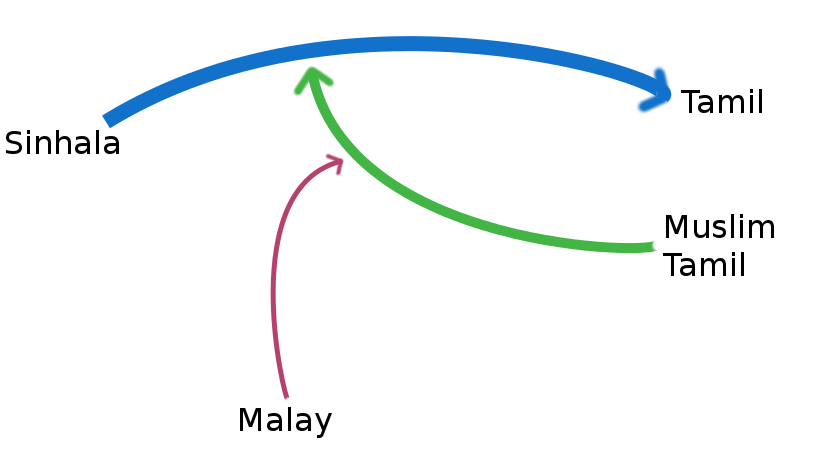
\includegraphics[height=.4\textheight]{changingdirections.png}
\caption{Illustration of the `directions' of language change. Sinhala changes towards Tamil, but Muslim Tamil changes towards Sinhala. Sri Lanka Malay changes towards Muslim Tamil and/or Sinhala.}
\end{figure}

\section{Discussion} \label{sec:discussion}
We started this paper by alluding to the open question whether Sri Lanka Malay was more influenced by Tamil or by Sinhala. The discussion of the dialectal situation on the island has shown that the question is actually more complicated, because Tamil, and even Moorish Tamil, shows internal dialectal variation which is more complex than previously assumed. Especially, South-Western Muslim Tamil is heavily influenced by Sinhala, which makes disentangling the respective influences even more difficult. While it is of course possible to claim that one language had a more important influence than the other, the intricate dialectal situation makes it difficult to see how influence of any of the languages could be discarded on structural grounds. 
The null hypothesis would remain that both languages exerted some influence, whether jointly (during periods of trilingualism) or separately, in successive layers of bilingualism of Malay + X \citep[cf.][]{Nordhoff2012xcmultilayer}.

Next to this rather pessimistic outlook, a further, more theoretically relevant point is that there are no fixed targets in language contact. Inert targets are of course tempting as they make the analysis more succinct. But as the examples of Sinhala moving towards Tamil, and South-Western Tamil moving towards Sinhala, have shown, at least in Sri Lanka, we are dealing with moving targets.  

\citet{Mattheier1996} argued that the term `convergence' is often mistaken, because usually there is one language which changes towards the other, while the target language is not at all influenced in return. He proposes that `advergence' might be a better term for one language asymptotically approaching another one. In the Sri Lankan case, it appears that we have several layers of advergence. Sinhala adverges towards a general Dravidian model, exemplified by Hindu/Christian varieties of Tamil. These varieties of Tamil do not change towards Sinhala. South-Western Muslim Tamil\footnote{And
 Negombo Tamil.
} adverges towards Sinhala, while Sinhala is not influenced in return by the Muslim dialect. Sri Lanka Malay, finally, changes towards both Sinhala and SW Muslim Tamil, while the latter varieties are not influenced by SLM.\footnote{Mathematically
 speaking, Sinhala $\to$ Tamil can be seen as an asymptote and SW Muslim Tamil $\to$ Sinhala as a curvilinear asymptote. The terms `advergence' and `asymptote' cannot be applied to the SLM  $\to$ SWMT/Sinhala case, as there are two targets, Sinhala and SW Muslim Tamil.
}
Mattheier's rejection of the term `convergence' is sensible for the Sri Lankan situation, where it is not the case that the languages all move towards a common goal where they would meet. But `advergence' in its original sense does not seem to be a very good term either, as this term suggests that there are languages which do not move. What we are dealing with in Sri Lanka is rather a case of `catch me if you can', where every target language is in turn on its way of trying to catch up with yet another language. 

% importance of a closer look into dialects and sociolects (threskeiolects)

% Kupwar
% 
% Standard Tamil (whether Sri Lankan or even Indian) is not at all part of the equation. 





\section{Conclusion}
Sri Lanka Malay has acquired many Dravidian structures. These structures do not stem from Standard Tamil, but either from Sinhala or South-Western Muslim Tamil.
Information about dialects and sociolects in Sri Lanka has improved our understanding of the language change processes going on on the island. We are now able to see that most varieties are moving, but that they do not share a common goal (i.e. convergence). Rather, every variety has its own target, and may in turn be target for yet another variety. We are not dealing with inert, static targets; instead the target languages are moving themselves. This makes the language change processes more difficult to model or analyze, but at the same time it gives good insights into the dynamics of Sri Lankan languages. 

\bibliographystyle{natmpi}
\bibliography{malay,nordhoffcollated,sinhala,tamil,lgctct,lgchg,creole,india,lankahist,ansaldo,sociolgstcs} 

\section*{Abbreviations}
\begin{tabular}{>{\sc}ll}
acc &  accusative\\
agr &  agreement \\
assoc & associative \\
cp  &    conjunctive participle\\
dat &  dative \\
dubit &  dubitative \\
inanim  & inanimate \\
indef  & indefinite\\ 
inf &  infinitive\\  
loc  & locative\\ 
pl &  plural \\
pres &  present \\
ptcp  & participle\\ 
quot &  quotative \\ 
\end{tabular}
\end{document}
 

 
  

 
 